\RequirePackage{fix-cm}
\documentclass[10pt,a4paper]{article}
\usepackage[T1]{fontenc}
\usepackage[default]{sourcesanspro}
\usepackage[margin=15mm]{geometry}
\usepackage{microtype}
\usepackage{enumitem}
\usepackage{titlesec}
\usepackage{xcolor}
\usepackage{etoolbox}
\usepackage{graphicx}
\usepackage{needspace}
\usepackage[backend=biber,style=ieee,sorting=site,defernumbers=true,maxbibnames=99,doi=true,url=false,isbn=false,giveninits=false]{biblatex}
\DeclareSortingTemplate{site}{\sort{\field{sortkey}}\sort{\field{year}}\sort{\field{title}}}
\definecolor{accent}{HTML}{254F70}
\usepackage[colorlinks=true,urlcolor=accent,linkcolor=accent,citecolor=accent]{hyperref}
\addbibresource{../assets/bibliography/publications.bib}
\setlength{\parindent}{0pt}
\setlength{\parskip}{2pt}
\setlist[itemize]{leftmargin=1.2em,nosep,topsep=3pt}
\titleformat{\section}{\fontsize{12}{14}\selectfont\bfseries\color{accent}}{}{0pt}{}[\titlerule]
\titlespacing*{\section}{0pt}{7pt}{3pt}
% Group headings stay close to the first citation; item spacing is independent.
\defbibheading{subbibliography}[\refname]{\needspace{3\baselineskip}\par\addvspace{3pt}{\fontsize{10}{12}\selectfont\bfseries #1}\par\nobreak}
\defbibenvironment{bibliography}
  {\list
     {\printtext[labelnumberwidth]{\printfield{labelprefix}\printfield{labelnumber}}}
     {\setlength{\labelwidth}{\labelnumberwidth}%
      \setlength{\leftmargin}{\labelwidth}%
      \setlength{\labelsep}{\biblabelsep}%
      \addtolength{\leftmargin}{\labelsep}%
      \setlength{\topsep}{0pt}%
      \setlength{\partopsep}{0pt}%
      \setlength{\itemsep}{\bibitemsep}%
      \setlength{\parsep}{\bibparsep}}%
   \renewcommand*{\makelabel}[1]{\hss##1}}
  {\endlist}
  {\item}
\pagestyle{empty}
\setlength{\bibitemsep}{3pt}
\renewcommand*{\bibfont}{\fontsize{9.5}{11}\selectfont}
\newcommand{\highlightself}[1]{\ifboolexpr{test {\ifdefstring{\namepartfamily}{Wu}} and test {\ifdefstring{\namepartgiven}{Zeming}}}{\textbf{#1}}{#1}}
\renewcommand*{\mkbibnamefamily}[1]{\highlightself{#1}\ifitemannotation{equal}{\textsuperscript{\ensuremath{\dagger}}}{}}
\renewcommand*{\mkbibnamegiven}[1]{\highlightself{#1}}
\DeclareFieldFormat{addendum}{{\color{accent}\footnotesize #1}}
\hypersetup{pdftitle={Zeming Wu - Academic CV},pdfauthor={Zeming Wu},pdfsubject={Robotics, distributed optimization, and motion planning}}

\begin{document}
\begin{minipage}[t]{0.83\linewidth}
% Spread the three text groups to match the portrait’s visible height.
\setlength{\parskip}{8.3pt}
\vspace{0pt}
{\LARGE\bfseries Zeming Wu}\par
PhD Candidate, Department of Mechanical Engineering\\
City University of Hong Kong, Hong Kong SAR, China\par
\small
\href{mailto:zeming.wu@my.cityu.edu.hk}{zeming.wu@my.cityu.edu.hk}
\enspace | \enspace \href{https://zamesng.github.io/}{Website}
\enspace | \enspace \href{https://scholar.google.com/citations?user=sMCRzUIAAAAJ}{Google Scholar}\\
\href{https://github.com/ZamesNg}{GitHub: ZamesNg}
\enspace | \enspace \href{https://www.linkedin.com/in/zeming-wu-439b661a9}{LinkedIn}
\enspace | \enspace \href{https://orcid.org/0009-0004-8751-6938}{ORCID: 0009-0004-8751-6938}
\end{minipage}\hfill
\begin{minipage}[t]{22mm}
\vspace{0.4pt}
% The source is already almost 4:5; trim only the fractional excess height.
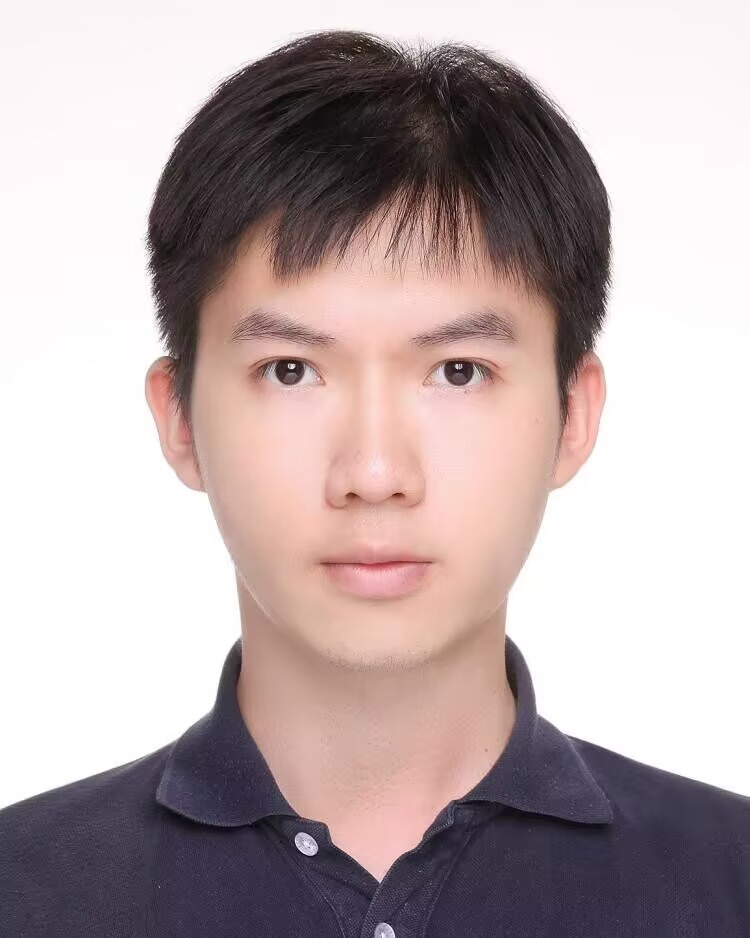
\includegraphics[width=22mm,height=27.5mm,trim=0 0.25bp 0 0.25bp,clip]{../assets/img/zeming-wu-cv.jpg}
\end{minipage}

\section{Education}
\begingroup
\setlength{\parskip}{6pt}
\needspace{3\baselineskip}
\textbf{City University of Hong Kong} --- Hong Kong SAR, China \hfill Sep 2024--Jun 2028 (Expected)\\
PhD in Mechanical Engineering; advisor: Prof. Lu Liu

\needspace{4\baselineskip}
\textbf{Tongji University} --- Shanghai, China \hfill Sep 2021--Jun 2024\\
M.Sc. in Control Science and Engineering\\
Supervisor: Prof. Zhuping Wang; research collaboration with Prof. Hao Zhang

\needspace{3\baselineskip}
\textbf{Tongji University} --- Shanghai, China \hfill Sep 2017--Jun 2021\\
B.Sc. in Automation\par
\endgroup

\section{Publications}
{\footnotesize\itshape Journal quartiles: JCR 2025 JIF, June 2026 release.}\par
\nocite{*}
\printbibliography[heading=subbibliography,title={First-author publications},keyword=first]
\printbibliography[heading=subbibliography,title={Co-first-author publications},keyword=cofirst]
\printbibliography[heading=subbibliography,title={Other publications},keyword=other]

\section{Research Interests}
Distributed optimization, trajectory optimization, and motion planning for multi-agent systems;
geometry-aware collision avoidance, robot coordination, and formation control.

\section{Technical Skills}
\textbf{Programming and machine learning:} Python, C/C++, MATLAB, PyTorch.\par
\textbf{Robotics software and simulators:} MuJoCo, Isaac Gym, PyBullet, ROS, ROS 2, Gazebo.\par
\textbf{Manipulators:} Franka FR3, AIRBOT Play.\par
\textbf{Mobile platforms:} Genisom M1 quadruped; PX4-based quadrotors; Crazyflie platforms; ground vehicles.

\section{Languages}
Mandarin (Native), Cantonese (Native), English.

\section{Reviewing Service}
\textbf{Journals:} T-RO, RA-L, T-AC, T-IE, T-II. \qquad \textbf{Conferences:} ICRA, IROS, CDC.
\end{document}
